\documentclass{article}
\usepackage{graphicx} % Required for inserting images
\usepackage[polish]{babel}
\usepackage[T1]{fontenc}
\usepackage{amsmath}
\usepackage{minted}
\graphicspath{{./images/}}

\title{Algorytmy macierzowe - Mnożenie macierzy}
\author{Jakub Frączek \and Kacper Garus}

\begin{document}

\sloppy

\maketitle

\tableofcontents

\newpage

\section{Wstęp}

Tematem zadania było wygenerowalnie losowych macierzy o wartościach z przedziału otwartego \((0.00000001, 1.0)\), a następnie zaimplementowanie algorytmów:

\begin{enumerate}
    \item Rekurencyjnego mnożenia macierzy metodą Binét’a
    \item Rekurencyjnego mnożenia macierzy metodą Strassena
    \item Mnożenia macierzy metodą AI na podstawie artykułu w Nature\(^*\)
\end{enumerate}

\noindent
* - https://deepmind.google/discover/blog/discovering-novel-algorithms-with-alphatensor/\#:~:text=In\%20our\%20paper,\%20published\%20today\%20in\%20Nature,\%20we

\bigbreak
\noindent
Następnie zliczyć liczbę operacji zmienno-przecinkowych dokonaną podczas mnożenia macierzy. Algorytmy miały zostać zaprojektowane tak, aby przyjmować macierze o dowolnych wymiarach.

\section{Metoda Binét’a}

\subsection{Opis teoretyczny}

Algrorytm Binét'a jest rekurencyjny i można go przedstawić dla przykładowych macierzy A i B w taki sposób:

\[
A =
\begin{bmatrix}
A_{11} & A_{12} \\
A_{21} & A_{22}
\end{bmatrix}
\quad
B =
\begin{bmatrix}
B_{11} & B_{12} \\
B_{21} & B_{22}
\end{bmatrix}
\]

\[
C =
\begin{bmatrix}
(A_{11}B_{11} + A_{12}B_{21}) & (A_{11}B_{12} + A_{12}B_{22}) \\
(A_{21}B_{11} + A_{22}B_{21}) & (A_{21}B_{12} + A_{22}B_{22})
\end{bmatrix}
\]

\bigbreak
\noindent
Gdzie \(A_{ij}\), \(B_{ij}\) dla \(i = {1, 2, ..., n}\) i \({j = {1, 2, ..., n}}\), to macierze


\subsection{Pseudokod}

\begin{minted}[bgcolor=white]{python}
Funkcja Binet(A, B)
    Jeżeli rozmiar(A) == 1
        Zwróć A * B

    środek = dzielenie_całkowite(rozmiar(A[0]), 2) 
    
    a11 = Wiersze od 0 do środek, Kolumny od 0 do środek z macierzy A
    a12 = Wiersze od 0 do środek, Kolumny od środek do n z macierzy A
    a21 = Wiersze od środek do n, Kolumny od 0 do środek z macierzy A
    a22 = Wiersze od środek do n, Kolumny od środek do n z macierzy A
    
    b11 = Wiersze od 0 do środek, Kolumny od 0 do środek z macierzy B
    b12 = Wiersze od 0 do środek, Kolumny od środek do n z macierzy B
    b21 = Wiersze od środek do n, Kolumny od 0 do środek z macierzy B
    b22 = Wiersze od środek do n, Kolumny od środek do n z macierzy B

    c11 = Binet(a11, b11) + Binet(a12, b21)
    c12 = Binet(a11, b12) + Binet(a12, b22)
    c21 = Binet(a21, b11) + Binet(a22, b21)
    c22 = Binet(a21, b12) + Binet(a22, b22)

    Zwróć macierz C złożóną z c11, c12, c21, c22
\end{minted}

\subsection{Implementacja}

Algorytm postanowiliśmy zaimplementować w języku Python:

\begin{minted}[bgcolor=white]{python}
def binet(a,b):
    
    if np.size(a)==1:
        return a*b
    n=np.size(a[0])
    mid=n//2
    
    a11=a[:mid,:mid]
    a12=a[:mid,mid:]
    a21=a[mid:,:mid]
    a22=a[mid:,mid:]
    b11=b[:mid,:mid]
    b12=b[:mid,mid:]
    b21=b[mid:,:mid]
    b22=b[mid:,mid:]

    c11=binet(a11, b11)+binet(a12, b21)
    c12=binet(a11, b12)+binet(a12, b22)
    c21=binet(a21, b11)+binet(a22, b21)
    c22=binet(a21, b12)+binet(a22, b22)

    return np.vstack((np.hstack((c11,c12)),np.hstack((c21,c22))))
\end{minted}

\section{Metoda Strassena}

\subsection{Opis teoretyczny}

Algorytm Strassena jest rekurencyjny i można go przedstawić dla przykładowych macierzy A i B w następujący sposób:

\[
A =
\begin{bmatrix}
A_{11} & A_{12} \\
A_{21} & A_{22}
\end{bmatrix}
\quad
B =
\begin{bmatrix}
B_{11} & B_{12} \\
B_{21} & B_{22}
\end{bmatrix}
\]

\[
C =
\begin{bmatrix}
P_{1} + P_{4} - P_{5} + P_{7} & P_{2} + P_{4} \\
P_{3} + P_{5} & P_{1} - P_{2} + P_{3} + P_{6}
\end{bmatrix}
\]

\[
\begin{aligned}
P_1 & = (A_{11} + A_{22})(B_{11} + B_{22}) & P_2 & = (A_{21} + A_{22})B_{11} \\
P_3 & = A_{11}(B_{12} - B_{22}) & P_4 & = A_{22}(B_{21} - B_{11}) \\
P_5 & = (A_{11} + A_{12})B_{22} & P_6 & = (A_{21} - A_{11})(B_{11} + B_{12}) \\
P_7 & = (A_{12} - A_{22})(B_{21} + B_{22}) &
\end{aligned}
\]

Gdzie \(A_{ij}\), \(B_{ij}\) dla \(i = {1, 2, ..., n}\) i \({j = {1, 2, ..., n}}\), to macierze

\subsection{Pseudokod}

\begin{minted}[bgcolor=white]{python}
Funkcja Binet(A, B)
    Jeżeli rozmiar(A) == 1
        Zwróć A * B

    środek = dzielenie_całkowite(rozmiar(A[0]), 2) 
    
    a11 = Wiersze od 0 do środek, Kolumny od 0 do środek z macierzy A
    a12 = Wiersze od 0 do środek, Kolumny od środek do n z macierzy A
    a21 = Wiersze od środek do n, Kolumny od 0 do środek z macierzy A
    a22 = Wiersze od środek do n, Kolumny od środek do n z macierzy A
    
    b11 = Wiersze od 0 do środek, Kolumny od 0 do środek z macierzy B
    b12 = Wiersze od 0 do środek, Kolumny od środek do n z macierzy B
    b21 = Wiersze od środek do n, Kolumny od 0 do środek z macierzy B
    b22 = Wiersze od środek do n, Kolumny od środek do n z macierzy B

    p1 = strassen(a11+a22, b11+b22)
    p2 = strassen(a21+a22, b11)
    p3 = strassen(a11, b12-b22)
    p4 = strassen(a22, b21-b11)
    p5 = strassen(a11+a12, b22)
    p6 = strassen(a21-a11, b11+b12)
    p7 = strassen(a12-a22, b21+b22)

    c11=p1+p4-p5+p7
    c12=p3+p5
    c21=p2+p4
    c22=p1-p2+p3+p6

    Zwróć macierz C złożóną z c11, c12, c21, c22
\end{minted}

\subsection{Implementacja}

Algorytm Strassena również został zaimplementowany w języku Python:

\begin{minted}[bgcolor=white]{python}
def strassen(a,b):
    n=np.size(a[0])
    
    if n==1:
        return a*b
    mid=n//2
    
    a11=a[:mid,:mid]
    a12=a[:mid,mid:]
    a21=a[mid:,:mid]
    a22=a[mid:,mid:]
    b11=b[:mid,:mid]
    b12=b[:mid,mid:]
    b21=b[mid:,:mid]
    b22=b[mid:,mid:]

    p1 = strassen(a11+a22, b11+b22)
    p2 = strassen(a21+a22, b11)
    p3 = strassen(a11, b12-b22)
    p4 = strassen(a22, b21-b11)
    p5 = strassen(a11+a12, b22)
    p6 = strassen(a21-a11, b11+b12)
    p7 = strassen(a12-a22, b21+b22)

    c11=p1+p4-p5+p7
    c12=p3+p5
    c21=p2+p4
    c22=p1-p2+p3+p6

    return np.vstack((np.hstack((c11,c12)),np.hstack((c21,c22))))
\end{minted}

\section{Metoda AI}

\subsection{Opis teoretyczny}

Autorzy artykułu "Discovering novel algorithms with AlphaTensor" w Nature postanowili spojrzeć na problem mnożenia macierzy w inny sposób przekształcając go w grę z bardzo dużą liczbą możliwych ruchów, której ukończenie jest równoważne znalezieniu szukanej macierzy. A następnie za pomocą uczenia maszynowego nauczyli model AlphaTensor, jak w nią graćm a ten metodą prób i błędóœ zaczął odkrywać najpierw już znane algorytmy, takie jak metoda Binét’a oraz metoda Strassena, aż dokonał przełomu odkrywając sposób wymnożenia macierzy 4x5 przez macierz 5x5 szybciej niż to było dotychczas możliwe. Najprostszy znany algorytm wykonuje obliczenia przy użyciu 100 mnożeń, algorytm Strassena przy 80, a algorytm AI przy 76.
\bigbreak

\begin{figure}[H]
  \centering
    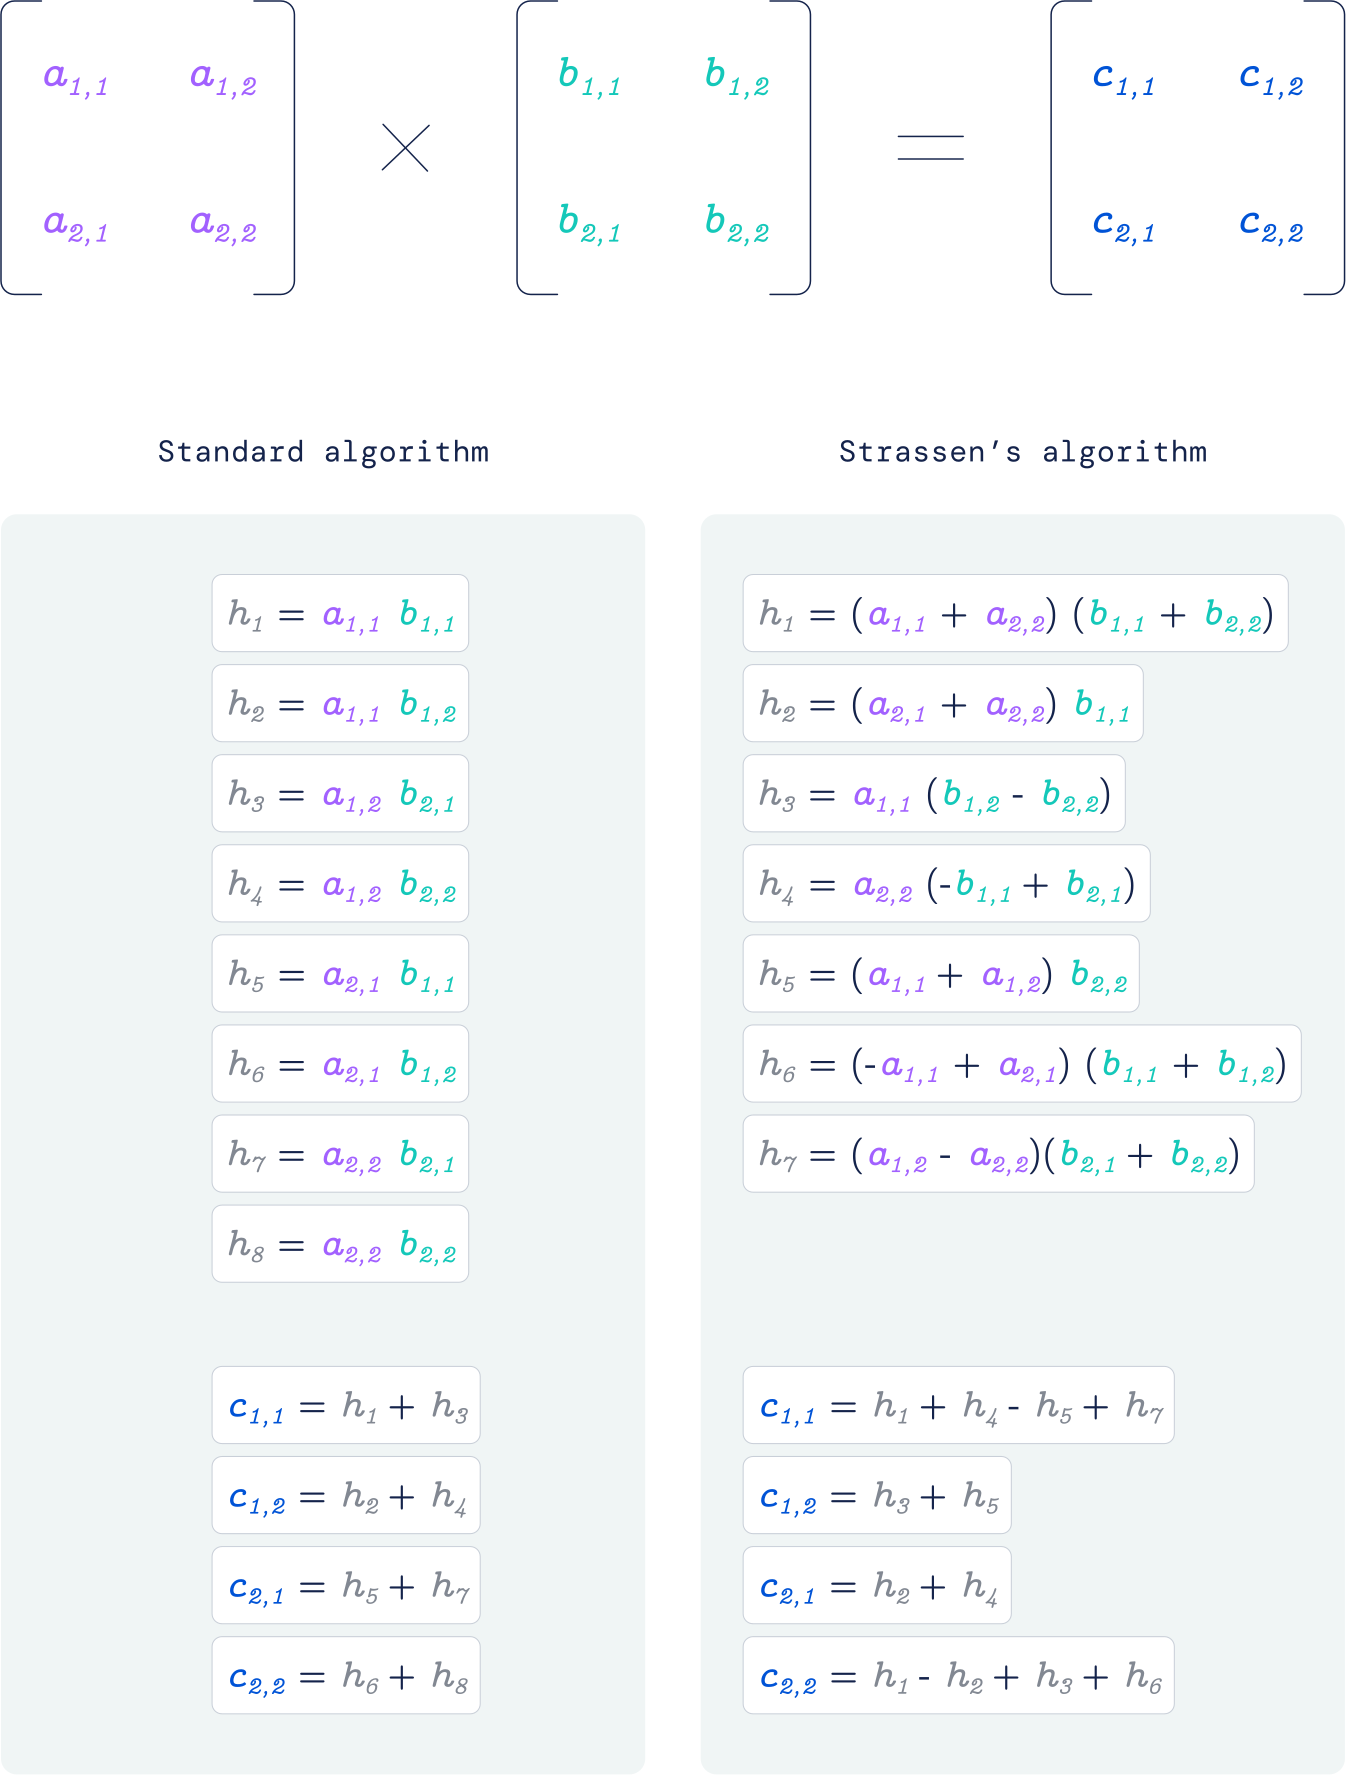
\includegraphics[width=0.7\textwidth]{images/standard_algorithms.png}
  \caption{Algoryty znane dotychczas}
\end{figure}

\begin{figure}[H]
  \centering
    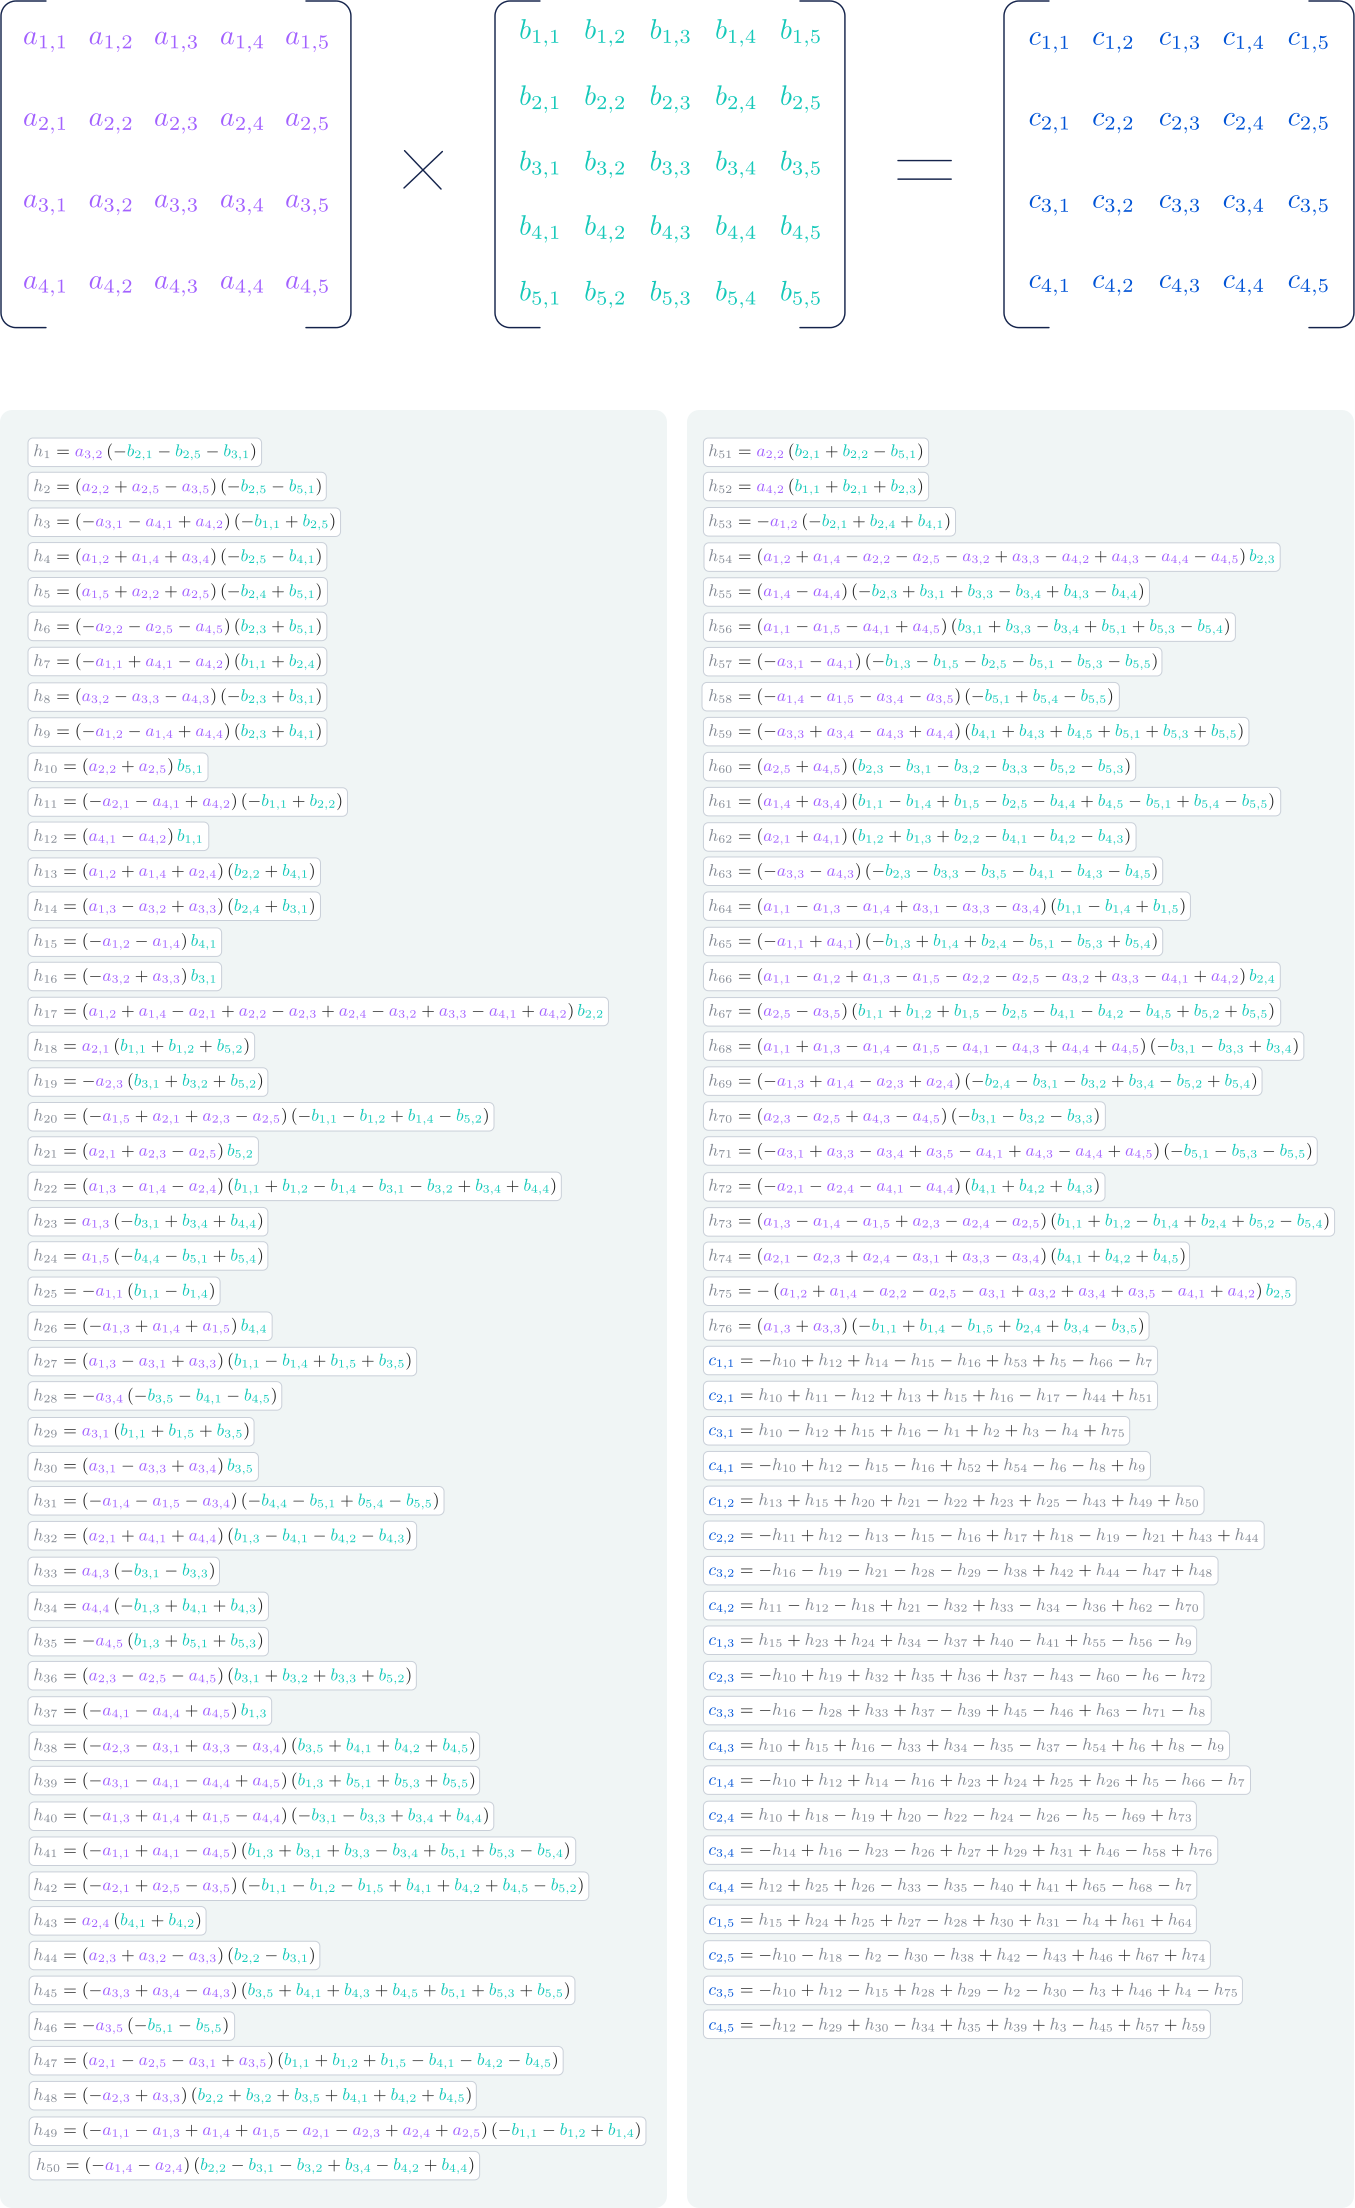
\includegraphics[width=0.99\textwidth]{AI.png}
  \caption{Algorytm wymyślony przez AI}
\end{figure}

\subsection{Implementacja}

Algorytm wymyśloney przez sztuczną inteligencję również został zaimplementowany w Pythonie:

\begin{minted}[bgcolor=white]{python}
def ai_matrix_mult(a,b):
    a11=a[0,0]
    a12=a[0,1]
    a13=a[0,2]
    a14=a[0,3]
    a15=a[0,4]
    a21=a[1,0]
    a22=a[1,1]
    a23=a[1,2]
    a24=a[1,3]
    a25=a[1,4]
    a31=a[2,0]
    a32=a[2,1]
    a33=a[2,2]
    a34=a[2,3]
    a35=a[2,4]
    a41=a[3,0]
    a42=a[3,1]
    a43=a[3,2]
    a44=a[3,3]
    a45=a[3,4]
    b11=b[0,0]
    b12=b[0,1]
    b13=b[0,2]
    b14=b[0,3]
    b15=b[0,4]
    b21=b[1,0]
    b22=b[1,1]
    b23=b[1,2]
    b24=b[1,3]
    b25=b[1,4]
    b31=b[2,0]
    b32=b[2,1]
    b33=b[2,2]
    b34=b[2,3]
    b35=b[2,4]
    b41=b[3,0]
    b42=b[3,1]
    b43=b[3,2]
    b44=b[3,3]
    b45=b[3,4]
    b51=b[4,0]
    b52=b[4,1]
    b53=b[4,2]
    b54=b[4,3]
    b55=b[4,4]

    h1=a32*(-b21-b25-b31)
    h2=(a22+a25-a35)*(-b25-b51)
    h3=(-a31-a41+a42)*(-b11+b25)
    h4=(a12+a14+a34)*(-b25-b41)
    h5=(a15+a22+a25)*(-b24+b51)
    h6=(-a22-a25-a45)*(b23+b51)
    h7=(-a11+a41-a42)*(b11+b24)
    h8=(a32-a33-a43)*(-b23+b31)
    h9=(-a12-a14+a44)*(b23+b41)
    h10=(a22+a25)*(b51)
    h11=(-a21-a41+a42)*(-b11+b22)
    h12=(a41-a42)*(b11)
    h13=(a12+a14+a24)*(b22+b41)
    h14=(a13-a32+a33)*(b24+b31)
    h15=(-a12-a14)*(b41)
    h16=(-a32+a33)*(b31)
    h17=(a12+a14-a21+a22-a23+a24-a32+a33-a41+a42)*(b22)
    h18=(a21)*(b11+b12+b52)
    h19=(-a23)*(b31+b32+b52)
    h20=(-a15+a21+a23-a25)*(-b11-b12+b14-b52)
    h21=(a21+a23-a25)*(b52)
    h22=(a13-a14-a24)*(b11+b12-b14-b31-b32+b34+b44)
    h23=(a13)*(-b31+b34+b44)
    h24=(a15)*(-b44-b51+b54)
    h25=(-a11)*(b11-b14)
    h26=(-a13+a14+a15)*(b44)
    h27=(a13-a31+a33)*(b11-b14+b15+b35)
    h28=(-a34)*(-b35-b41-b45)
    h29=(a31)*(b11+b15+b35)
    h30=(a31-a33+a34)*(b35)
    h31=(-a14-a15-a34)*(-b44-b51+b54-b55)
    h32=(a21+a41+a44)*(b13-b41-b42-b43)
    h33=(a43)*(-b31-b33)
    h34=(a44)*(-b13+b41+b43)
    h35=(-a45)*(b13+b51+b53)
    h36=(a23-a25-a45)*(b31+b32+b33+b52)
    h37=(-a41-a44+a45)*(b13)
    h38=(-a23-a31+a33-a34)*(b35+b41+b42+b45)
    h39=(-a31-a41-a44+a45)*(b13+b51+b53+b55)
    h40=(-a13+a14+a15-a44)*(-b31-b33+b34+b44)
    h41=(-a11+a41-a45)*(b13+b31+b33-b34+b51+b53-b54)
    h42=(-a21+a25-a35)*(-b11-b12-b15+b41+b42+b45-b52)
    h43=(a24)*(b41+b42)
    h44=(a23+a32-a33)*(b22-b31)
    h45=(-a33+a34-a43)*(b35+b41+b43+b45+b51+b53+b55)
    h46=(-a35)*(-b51-b55)
    h47=(a21-a25-a31+a35)*(b11+b12+b15-b41-b42-b45)
    h48=(-a23+a33)*(b22+b32+b35+b41+b42+b45)
    h49=(-a11-a13+a14+a15-a21-a23+a24+a25)*(-b11-b12+b14)
    h50=(-a14-a24)*(b22-b31-b32+b34-b42+b44)
    h51=(a22)*(b21+b22-b51)
    h52=(a42)*(b11+b21+b23)
    h53=(-a12)*(-b21+b24+b41)
    h54=(a12+a14-a22-a25-a32+a33-a42+a43-a44-a45)*(b23)
    h55=(a14-a44)*(-b23+b31+b33-b34+b43-b44)
    h56=(a11-a15-a41+a45)*(b31+b33-b34+b51+b53-b54)
    h57=(-a31-a41)*(-b13-b15-b25-b51-b53-b55)
    h58=(-a14-a15-a34-a35)*(-b51+b54-b55)
    h59=(-a33+a34-a43+a44)*(b41+b43+b45+b51+b53+b55)
    h60=(a25+a45)*(b23-b31-b32-b33-b52-b53)
    h61=(a14+a34)*(b11-b14+b15-b25-b44+b45-b51+b54-b55)
    h62=(a21+a41)*(b12+b13+b22-b41-b42-b43)
    h63=(-a33-a43)*(-b23-b33-b35-b41-b43-b45)
    h64=(a11-a13-a14+a31-a33-a34)*(b11-b14+b15)
    h65=(-a11+a41)*(-b13+b14+b24-b51-b53+b54)
    h66=(a11-a12+a13-a15-a22-a25-a32+a33-a41+a42)*(b24)
    h67=(a25-a35)*(b11+b12+b15-b25-b41-b42-b45+b52+b55)
    h68=(a11+a13-a14-a15-a41-a43+a44+a45)*(-b31-b33+b34)
    h69=(-a13+a14-a23+a24)*(-b24-b31-b32+b34-b52+b54)
    h70=(a23-a25+a43-a45)*(-b31-b32-b33)
    h71=(-a31+a33-a34+a35-a41+a43-a44+a45)*(-b51-b53-b55)
    h72=(-a21-a24-a41-a44)*(b41+b42+b43)
    h73=(a13-a14-a15+a23-a24-a25)*(b11+b12-b14+b24+b52-b54)
    h74=(a21-a23+a24-a31+a33-a34)*(b41+b42+b45)
    h75=-(a12+a14-a22-a25-a31+a32+a34+a35-a41+a42)*(b25)
    h76=(a13+a33)*(-b11+b14-b15+b24+b34-b35)

    c11=-h10+h12+h14-h15-h16+h53+h5-h66-h7
    c21=h10+h11-h12+h13+h15+h16-h17-h44+h51
    c31=h10-h12+h15+h16-h1+h2+h3-h4+h75
    c41=-h10+h12-h15-h16+h52+h54-h6-h8+h9
    c12=h13+h15+h20+h21-h22+h23+h25-h43+h49+h50
    c22=-h11+h12-h13-h15-h16+h17+h18-h19-h21+h43+h44
    c32=-h16-h19-h21-h28-h29-h38+h42+h44-h47+h48
    c42=h11-h12-h18+h21-h32+h33-h34-h36+h62-h70
    c13=h15+h23+h24+h34-h37+h40-h41+h55-h56-h9
    c23=-h10+h19+h32+h35+h36+h37-h43-h60-h6-h72
    c33=-h16-h28+h33+h37-h39+h45-h46+h63-h71-h8
    c43=h10+h15+h16-h33+h34-h35-h37-h54+h6+h8-h9
    c14=-h10+h12+h14-h16+h23+h24+h25+h26+h5-h66-h7
    c24=h10+h18-h19+h20-h22-h24-h26-h5-h69+h73
    c34=-h14+h16-h23-h26+h27+h29+h31+h46-h58+h76
    c44=h12+h25+h26-h33-h35-h40+h41+h65-h68-h7
    c15=h15+h24+h25+h27-h28+h30+h31-h4+h61+h64
    c25=-h10-h18-h2-h30-h38+h42-h43+h46+h67+h74
    c35=-h10+h12-h15+h28+h29-h2-h30-h3+h46+h4-h75
    c45=-h12-h29+h30-h34+h35+h39+h3-h45+h57+h59

    c=np.array([[c11,c12,c13,c14,c15],[c21,c22,c23,c24,c25],
               [c31,c32,c33,c34,c35],[c41,c42,c43,c44,c45]])
    
    return c
\end{minted}

\section{Test działania algorytmu AI}

W celu przetestowania poprawności algorytmu "wymyślonego" przez sztuczną inteligencję, wygenerowaliśmy dwie macierze z losowymi wartościami, a następni wymnożyliśmy je metodą AI oraz funkacją np.dot(). Po porównaniu otrzymanych wyników okazało się, że metoda jest poprawna, a różnica pomiędzy poszczególnymi elementami macierzy wynikowej jest minimalna i wynika stricte ze sposobu przechowywanie i operacji na liczbach zmiennoprzecinkowych w komputerze. Poniżej zamieściliśmy wykorzystane macierze oraz otrzymane różnice.

\[
A = \begin{bmatrix}
0.12 & 0.34 & 0.56 & 0.78 & 4.55 \\
1.23 & 1.45 & 1.67 & 1.89 & 4.66 \\
2.01 & 2.23 & 2.45 & 2.67 & 4.77 \\
3.11 & 3.22 & 3.33 & 3.44 & 4.88
\end{bmatrix}
\]

% Macierz B
\[
B = \begin{bmatrix}
0.10 & 0.20 & 0.30 & 0.40 & 0.50 \\
1.00 & 1.10 & 1.20 & 1.30 & 1.40 \\
2.00 & 2.10 & 2.20 & 2.30 & 2.40 \\
3.00 & 3.10 & 3.20 & 3.30 & 3.40 \\
4.00 & 4.10 & 4.20 & 4.30 & 4.40
\end{bmatrix}
\]

\[
C1 = C2 = A \cdot B
\]
Gdzie C1 to wynik otrzymany metodami AI, a C2 przy wykorzystaniu numpy
\[
C1 - C2 =
\begin{bmatrix}
3.55 \times 10^{-15} & 0.00 & 3.55 \times 10^{-15} & 7.11 \times 10^{-15} & 3.55 \times 10^{-15} \\
3.55 \times 10^{-15} & 3.55 \times 10^{-15} & 1.07 \times 10^{-14} & 7.11 \times 10^{-15} & 7.11 \times 10^{-15} \\
0.00 & 0.00 & 1.42 \times 10^{-14} & 0.00 & 0.00 \\
0.00 & 2.13 \times 10^{-14} & 0.00 & 0.00 & 1.42 \times 10^{-14}
\end{bmatrix}
\]


\section{Porównanie wydajności algorytmów Binet'a i Strassena}

\subsection{Zlliczanie liczby operacji zmiennoprzecinkowych}

Zliczanie operacji zmiennoprzecinkowych osiągnęliśmy poprzez stworzenie typu danych dziedziczącego po float'cie i przeładowującego operacje arytmetyczne tak aby ich wywołania były zliczane. Z uwagi na wybrany sposób implementacji warunków zadania (tj. wypełnianie macierzy zerami, tak aby liczba wirszy i kolumn była równa najbliższej większej potędze dwójki), po zmierzeniu liczby FLOPS'ów otrzymaliśmy 9 róznych zestawów wartości dla algorytmu Binet'a, co zostało zaprezentowane w tabeli 1.

\begin{table}[H]
    \centering
    \begin{tabular}{|l|l|l|l|l|}
    \hline
        Rozmiar macierzy & Mnożenia & Dodawania & Odejmowania & Dzielenia  \\ \hline
        2 & 8 & 4 & 0 & 0  \\ \hline
        4 & 64 & 48 & 0 & 0  \\ \hline
        8 & 512 & 448 & 0 & 0  \\ \hline
        16 & 4096 & 3840 & 0 & 0  \\ \hline
        32 & 32768 & 31744 & 0 & 0  \\ \hline
        64 & 262144 & 258048 & 0 & 0  \\ \hline
        128 & 2097152 & 2080768 & 0 & 0  \\ \hline
        256 & 16777216 & 16711680 & 0 & 0  \\ \hline
        512 & 134217728 & 133955584 & 0 & 0 \\ \hline
    \end{tabular}
    \caption{Liczba poszczególnych operacji zmiennoprzecinkowych dla algorytmu Binet'a}
\end{table}

\noindent
Na poniższym wykresie zaprezentowaliśmy sumaryczną liczbę operacji zmiennoprzecinkowych dla rozmiarów macierzy z zakresu od 1 do 512.

\begin{figure}[H]
  \centering
    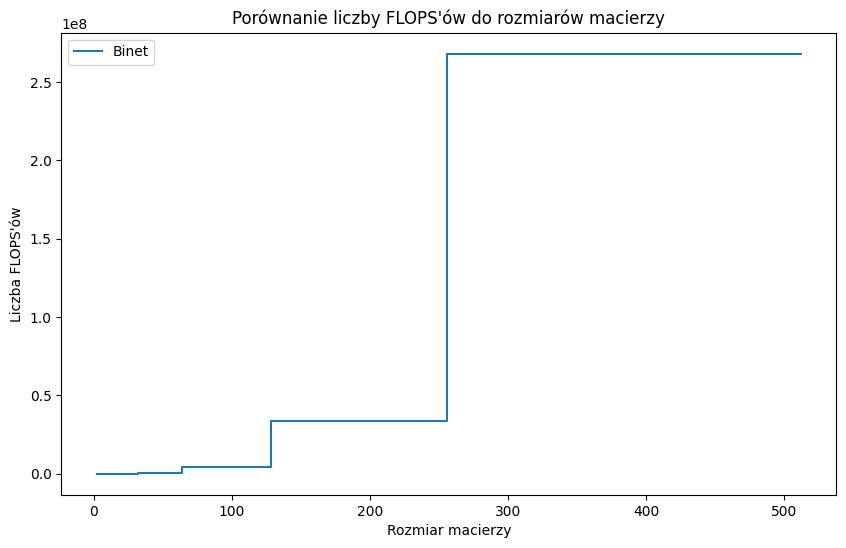
\includegraphics[width=0.8\textwidth]{binet_flops.png}
  \caption{Sumaryczna liczba FLOPS'ów dla algorytmu Binet'a}
\end{figure}

Taką samą analizę przeprowadziliśmy dla algorytmu Strassen'a również otrzymując 9 unikalnych zestawów wartości, co widać w tabeli poniżej.

\begin{table}[H]
    \centering
    \begin{tabular}{|l|l|l|l|l|}
    \hline
        Rozmiar macierzy & Mnożenia & Dodawania & Odejmowania & Dzielenia  \\ \hline
        2 & 7 & 12 & 6 & 0  \\ \hline
        4 & 49 & 132 & 66 & 0  \\ \hline
        8 & 343 & 1116 & 558 & 0  \\ \hline
        16 & 2401 & 8580 & 4290 & 0  \\ \hline
        32 & 16807 & 63132 & 31566 & 0  \\ \hline
        64 & 117649 & 454212 & 227106 & 0  \\ \hline
        128 & 823543 & 3228636 & 1614318 & 0  \\ \hline
        256 & 5764801 & 22797060 & 11398530 & 0  \\ \hline
        512 & 40353607 & 160365852 & 80182926 & 0 \\ \hline
    \end{tabular}
    \caption{Liczba poszczególnych operacji zmiennoprzecinkowych dla algorytmu Strassen'a}
\end{table}

\noindent
Ponownie sporządziliśmy wykres prezentujący sumaryczną liczbę FLOPS'ów dla macierzy o rozmiarach z zakresu od 1 do 512.

\begin{figure}[H]
  \centering
    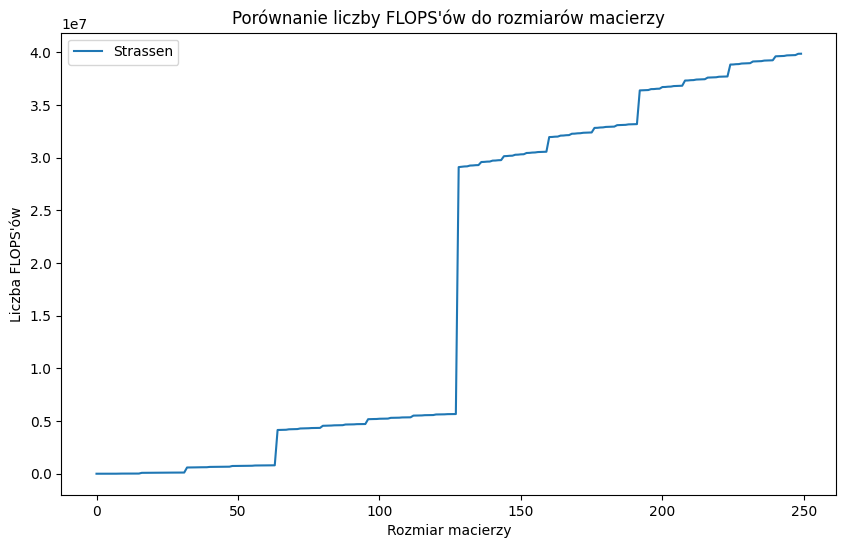
\includegraphics[width=0.8\textwidth]{images/strassen_flops.png}
  \caption{Sumaryczna liczba FLOPS'ów dla algorytmu Strassen'a}
\end{figure}

\subsection{Porównanie czasów działania}

Jak widać czasy wykonania znów tworzą schodkowy wykres, co wynika z faktu uzupełniania macierzy zerami. Osiągane wartości są dość duże, dla rozmiarów 257 - 250 było to już ok. 50s. Na wykresie można zobaczyć pik czasu wykonania dla rozmiarów macierzy pomiędzy 150 do 200, najprawdopodobniej wynika on poprostu z większego obciążenia procesora w tym czasie (Całość liczyła się ok. 100 minut). 

\begin{figure}[H]
  \centering
    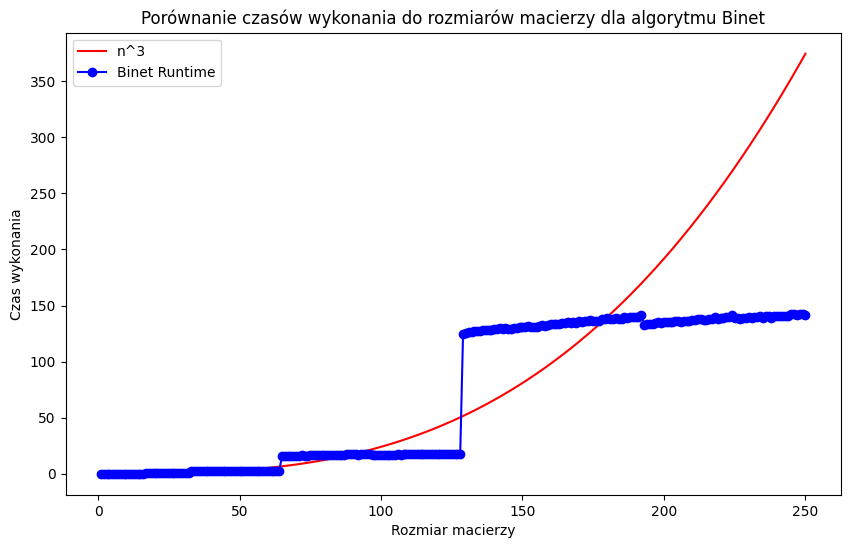
\includegraphics[width=0.8\textwidth]{images/binet_runtime.png}
  \caption{Wykres czasu działania algorytmu Binet'a dla różnych rozmiarów macierzy}
\end{figure}

\noindent
Podobnie sytuacja wygląda dla algorytmu Strassena, co widać na wykresie poniżej.

\begin{figure}[H]
  \centering
    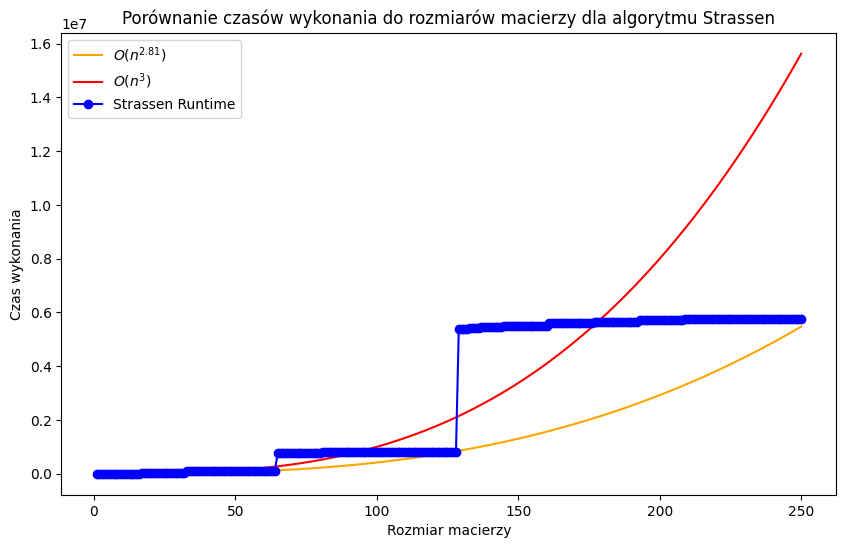
\includegraphics[width=0.8\textwidth]{images/strassen_runtime.png}
  \caption{Wykres czasu działania algorytmu Strassen'a dla różnych rozmiarów macierzy}
\end{figure}

\noindent
Sporządziliśmy jeszcze jeden wykres prezentujący oba czasy działania na jednym wykresie, co pięknie obrazuje niższą złożoność algorytmu Strassena.

\begin{figure}[H]
  \centering
    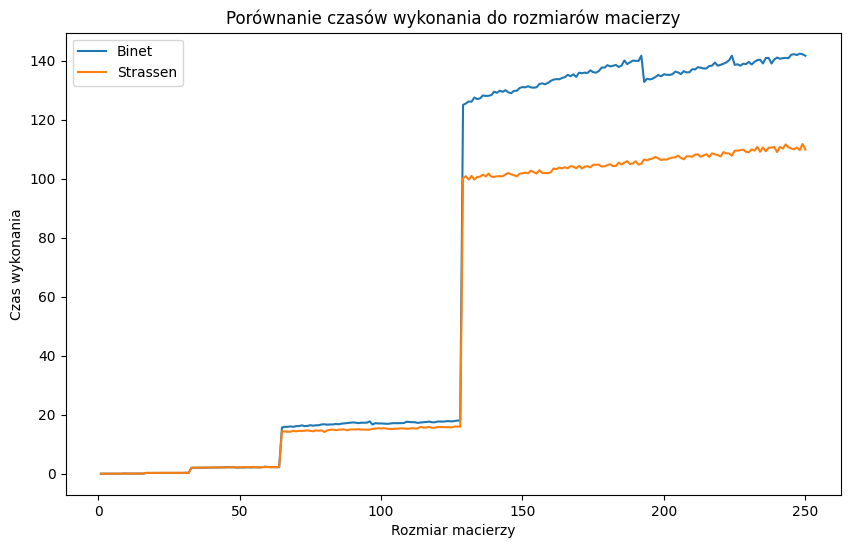
\includegraphics[width=0.8\textwidth]{images/binet_strassen_runtime.png}
  \caption{Porównanie czasów działania algorytmu Binet'a i Strassena}
\end{figure}

\section{Oszacowanie złożoności obliczeniowej}

Złożoność obliczeniową postanowiliśmy oszacować teoretycznie. Dla algorytmu Binét'a algorytm wykonuje 8 mnożeń na każdym etapie, a liczba podziałów wynosi \(log{2}[n]\), zatem liczba operacji wynosi \(8^{log{2}{n}} = n^3\). Jeśli chodzi o algorytm Strassena wykonuje on 7 mnożeń na każdym etapie, zatem złożoność wynosi \(7^{log{2}{n}} = n^{2.81}\).

\section{Porównanie wyników z Octave}

W celu sprawdzenia poprawności zaimplementowanych algorytmów porównaliśmy wyniki mnożenia 2 macierzy w Octave oraz za pomocą naszych implementacji algorytmu Binet'a i Strassena. Poniżej zamieszczony jest kod w Octave, który użyliśmy do pomnożenia macierzy.

\begin{minted}[bgcolor=white]{python}
A = [1.1, 2.2, 3.3, 7.1;
     4.4, 5.5, 6.6, 3.2;
     7.7, 8.8, 9.9, 5.1];

B = [9.9, 8.8, 7.7, 7.6;
     6.6, 5.5, 4.4, 6.2;
     3.3, 2.2, 1.1, 1.2];

C = A * B;

disp(C);
\end{minted}

\noindent
Wyniki otrzymane tymi trzeba sposobami były identyczne. Zaobserwowaliśmy, że implementacja mnożenia w Octave jest dużo lepsza i kod wykonuje się znacznie szybciej, niż w przypadku naszych algorytmów. Szczególnie przeprowadziliśmy testy dla macierzy 350x350. Kod w Octave wykonuje się w ułamku sekundy, gdzie nasza implementacja algorytmu Binet'a i Strassena potrzebuje paręset sekund.

\section{Wnioski}

\begin{enumerate}
    \item Algorytm Strassena jest szybszy od algorytmu Binet'a, co zostało przez nas pokazane teoretycznie jak i zaobserwowane podczas testów.
    \item Metoda mnożenia zaproponowana przez AI jest poprawna, jednak jej implementacja jest dość długa.
    \item Jednym z powodów dość powolnego mnożenia macierzy jest implementacja algorytmów w języku Python, prawdopodobnie dużo lepsze czasy uzyskalibyśmy implementując je w C.
    \item Octave nadaje się do mnożenia bardzo dużych macierzy.
\end{enumerate}

\end{document}
